\documentclass[border=6pt]{standalone}
\usepackage[T1]{fontenc}
\usepackage[utf8]{inputenc}
\usepackage{mathptmx}
\usepackage{amsmath,amssymb,amsfonts,mathrsfs}
\usepackage[dvipsnames]{xcolor}
\usepackage{tikz}
\usetikzlibrary{calc,positioning,arrows.meta,decorations.pathreplacing,
                decorations.markings,matrix,fit,backgrounds,shapes.misc}
\renewcommand{\sl}{\mathfrak{sl}}
\newcommand{\Uq}{U_q(\sl_2)}
\newcommand{\qint}[1]{[#1]_q}
\newcommand{\Rcheck}{\check{R}}
\definecolor{accent}{RGB}{59,91,146}
\definecolor{accentsoft}{RGB}{155,180,216}
\definecolor{oddsign}{RGB}{138,40,132}
\tikzset{
  strand/.style={line width=1pt, accent!80!black},
  rbox/.style={draw=accent!70!black, fill=accentsoft!55, rounded corners=2pt,
               line width=0.8pt, minimum height=6mm},
  rdot/.style={circle, fill=accent, inner sep=1.6pt},
  knode/.style={circle, draw=accent!70!black, fill=accentsoft!45,
                line width=0.8pt, minimum size=7mm, font=\small},
  kedge/.style={accent!70!black, line width=0.9pt},
  faredge/.style={oddsign!75!black, line width=0.9pt, densely dashed},
  glabel/.style={font=\footnotesize, accent!60!black},
}
\begin{document}
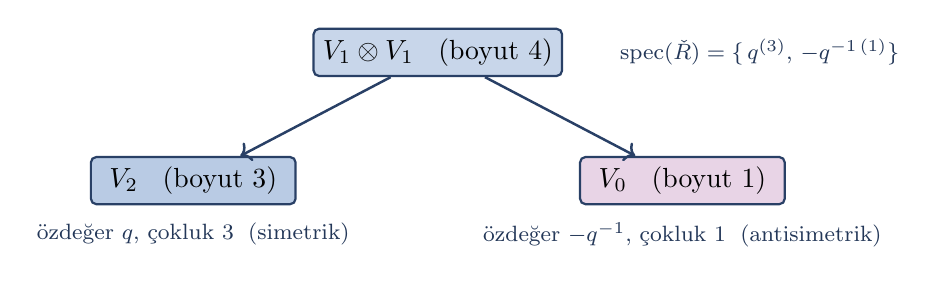
\begin{tikzpicture}[node distance=8mm]
  \node[rbox, minimum width=30mm] (vv) {$V_1\otimes V_1$\;\; (boyut 4)};
  \node[rbox, fill=accentsoft!70, minimum width=26mm, below left=10mm and 2mm of vv] (v2)
    {$V_2$\;\; (boyut 3)};
  \node[rbox, fill=oddsign!20, minimum width=26mm, below right=10mm and 2mm of vv] (v0)
    {$V_0$\;\; (boyut 1)};
  \draw[kedge,->] (vv) -- (v2);
  \draw[kedge,->] (vv) -- (v0);
  \node[glabel, below=1mm of v2] {özdeğer $q$, çokluk 3 \;(simetrik)};
  \node[glabel, below=1mm of v0] {özdeğer $-q^{-1}$, çokluk 1 \;(antisimetrik)};
  \node[glabel, accent!60!black, right=6mm of vv, align=left]
    {$\mathrm{spec}(\Rcheck)=\{\,q^{(3)},\,-q^{-1\,(1)}\}$};
\end{tikzpicture}
\end{document}
